\documentclass[../bccalc.tex]{subfiles}
\graphicspath{{\subfix{../figures/}}}
\begin{document}
\chapter{Integration with Data, Functions Defined by Integrals, and Natural Logs}
\section{Integration Using Data}
\begin{example}
    Water is flowing into a tank over a 24-hour period. The rate at which water is flowing into the tank at various times is measured, and the results are given in the table below, where $R(t)$ is measured in gallons per hour and $t$ is measured in hours. The tank contains 150 gallons of water when $t=0$.
    \begin{center}
        \begin{tabular}{|c|c|c|c|c|c|c|c|}
            \hline
            $t$ (hours) & 0 & 4 & 8 & 12 & 16 & 20 & 24 \\ \hline 
            $R(t)$ (gal/hr) & 8 & 8.8 & 9.3 & 9.2 & 8.9 & 8.1 & 6.7 \\ \hline
        \end{tabular}
    \end{center}
    (a) Estimate the number of gallons of water in the tank at the end of 24 hours by using a midpoint Riemann sum with three subintervals and values from the table. Show the computations that lea dto your answer.

    We are estimating $150+\int_0^{24} R(t)dt=W(24)-W(0)$.

    So $150+[3(8.8)+8(9.2)+8(8.1)]=358.8$ gallons

    (b) Estimate the number of gallons of water in the tank at the end of 24 hours by using a trapezoidal sum with three subintervals and values from the table. Show the computations that lead to your answer.

    This is $150+\left[8\left(\frac{8+9.3}{2}\right)+8\left(\frac{9.3+8.9}{2}\right)+8\left(\frac{8.9+6.7}{2}\right) \right] = 354.4$ gallons.

    (c) A model for this function is given by $W(t)=\frac{1}{75}(600+20t-t^2)$. Use the model to find the number of gallons of water in the tank at the end of 24 hours.

    $\int_0^{24}w(t)dt=W(24)-W(0)$.

    $150+\int_0^{24}W(t)dt = 357.36$

    (d) Use the model given in (c) to find the average rate of water flow over the 24-hour period.

    $\frac{1}{24-0}\int_0^{24}W(t)dt = 8.64$ gallons/hr
\end{example}

\section{Second Fundamental Theorem of Calculus}
Let us investigate first.

Find $\frac{d}{dx}\int_1^x t^2 dt$. This is equal to $x^2$.

Find $\frac{d}{dx}\int_{\pi/6}^x \cos t dt$. This is equal to $\cos x$.

See a pattern?

\begin{theorem}[Second Fundamental Theorem of Calculus]
    \[ \frac{d}{dx}\int_a^x f(t)dt=f(x)\]
\end{theorem}

\pagebreak
\begin{example}
    \[ \frac{d}{dx}\int_x^4 t^2 dt \]

    This is $-\frac{d}{dx}\int_4^x t^2 dt = -x^2$
\end{example}

In general, $\frac{d}{dx}\int_x^a f(t)dt = -f(x)$.

\begin{example}
    \[ \frac{d}{dx}\int_{\pi/6}^{x^2} \cos t dt \]

    This is $\frac{d}{dx}[\sin t]$ with bounds $\pi/6$ to $x^2$.

    We end up getting $\frac{d}{dx}[\sin (x^2)-\frac{1}{2}]=\cos (x^2)\cdot 2x$.
\end{example}

\begin{theorem}[Second Fundamental Theorem of Calculus]
    \[ \frac{d}{dx}\int_a^{g(x)}f(t)dt = f(g(x))\cdot g'(x) \]
\end{theorem}

\begin{example}
    Use the Second Fundamental Theorem to evaluate.

    (a) $\frac{d}{dx}\int_3^x \sqrt{1+t^2}dt$

    This is $\sqrt{1+x^2}$

    (b) $\frac{d}{dx}\int_2^x \tan(t^3)dt$

    This is $\tan(x^3)$.
\end{example}

\ex Same as above for $\frac{d}{dx}\int_{-1}^{x^3}\frac{1}{1+t}dt$

\ex Same as above for $\frac{d}{dx}\int_2^{\sin x}\sqrt[3]{1+t^2}dt$
\pagebreak
\begin{example}
    The graph of a function $f$ consists of a quarter circle and line segments. Let $g$ be the function given by 
    \[ g(x)=\int_0^x f(t)dt \]
    \begin{center}
    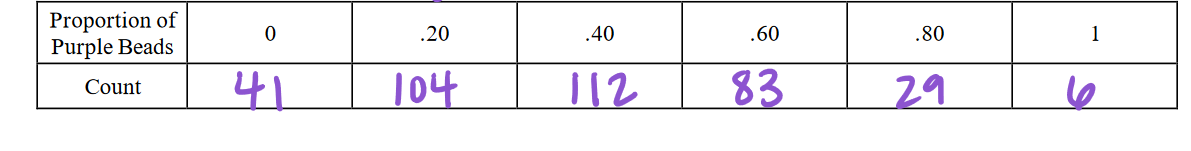
\includegraphics[width=0.3\textwidth]{5.1.1.PNG}
\end{center}
(a) Find $g(0), g(-1), g(2), g(5)$

$g(0)=\int_0^0 f(t)dt =0 $

$g(-1)=\int_0^{-1}f(t)dt = -\int_{-1}^0 f(t)dt = -1$

$g(2)=\int_0^2 f(t)dt = \pi$

$g(5) = \int_0^5 f(t)dt = \pi-4$

(b) Find all values of $x$ on the open interval $(-1,5)$ at which $g$ has a relative maximum. Justify your answer.

$g'(x) = f(x)$ crosses the $x$-axis from positive to negative at $x=2$.
\end{example}

\ex Using the information above, (c) Find the absolute minimum value of $g$ on $[-1,5]$ and the value of $x$ at which it occurs. Justify your answer.

\ex Using the information above, (d) Find the $x$-coordinate of each point of inflection of the graph of $g$ on $(-1,5)$. Justify your answer.

\section{Natural Logs and Differentiation}
\begin{definition}[Natural Logarithmic Function]
    The natural logarithmic function is defined by $\ln x = \int_1^x \frac{1}{t}dt$ where $x>0$.
\end{definition}

The base of natural logs is the number $e$. $e$ was named for a Swiss mathematician, Leonhard Euler.

By definition: 
\[ e = \lim_{n\to \infty}\left(1+\frac{1}{n}\right)^n = \lim_{n\to \infty}\left(\frac{n+1}{n}\right)^n \approx 2.7183\dots \]

$y=\ln x$ and $y=e^x$ are inverses.

Properties of Natural Logs:
\begin{enumerate}
    \item Domain of $y=\ln x$ is $(0,\infty)$. Range of $y=\ln x$ is $(-\infty,\infty)$.
    \item The graph of $y=\ln x$ is continuous, increasing, and one-to-one 
    \item The graph of $y=\ln x$ is concave down.
\end{enumerate}

Other properties:

    If $a$ and $b$ are positive numbers and $n$ is rational, then:
\begin{enumerate}
    \item $\ln 1 = 0$
    \item $\ln e = 1$
    \item $\ln ab = \ln a + \ln b$
    \item $\ln \frac{a}{b}=\ln a - \ln b$
    \item $\ln a^n = n\ln a$
\end{enumerate}

\ex Write as a sum, difference, or multiple of logs: $\ln \frac{(x^2+3)^2}{\sqrt[3]{x^2+1}}$

\ex Write as a single log: $2\ln (x+3)+\frac{1}{2}\ln (x-2)$

\begin{definition}
    \[ \frac{d}{dx}[\ln u]=\frac{1}{u}\frac{du}{dx}, u>0 \]
\end{definition}

\begin{example}
    If $y=\ln (2x)$, what is $y'$.

    $y'=\frac{1}{2x}\cdot 2 = \frac{1}{x}$.
\end{example}

\ex Find $f'(x)$ if $f(x)=\ln(x^2+1)$

\ex Find $y'$ if $y=x\ln x$

\ex Find $f'(x)$ if $f(x)=\ln\sqrt{x+1}$

\ex Find $y'$ if $y=\ln(\ln x)$

\ex Find $y'$ if $y=\ln(x^3)$

\ex Find $y'$ if $y=(\ln x)^3$

\begin{example}
    Show that $y=x\ln x-4x$ is a solution to the differential equation 
    \[ x+y-xy'=0 \]

    $y'=-3+\ln x$, so plugging this in gives $x+(x\ln x-4x)-x(-3+\ln x)=0$.

    Everything cancels out and we see that $0=0$ which is true.
\end{example}

\section{The Natural Log Function and Integration}
We previously saw differentiation.

Now integration.
\[ \int \frac{1}{u}du = \ln|u|+C \]

\begin{example}
    $\int \frac{2}{x}dx$

    Simple! This is $2\ln |x|+C$.    
\end{example}

\ex $\int_1^e \frac{2}{x}dx$

\ex $\int \frac{1}{2x-1}dx$

\ex $\int \frac{3x^2+1}{x^3+x}dx$

\ex $\int_1^e \frac{(1+\ln x)^3}{x}dx$

\ex $\int_e^{e^2}\frac{(\ln x)^4}{x}dx$

\ex $\int_0^3 \frac{x^2-5}{x+2}dx$

If you are integrating a quotient and the power of the numerator is greater than or equal to the power of the denominator you must divide.

Four more integration formulas:
\begin{itemize}
    \item $\int \tan u du = -\ln|\cos u|+C$
    \item $\int \cot u du = \ln|\sin u|+C$
    \item $\int \sec u du = \ln|\sec u + \tan u|+C$
    \item $\int \csc u du = -\ln|\csc u + \cot u|+C$
\end{itemize}

\begin{example}
    Why is $\int \tan x dx = -\ln|cos x|+C$ true?

    Let $\int \frac{\sin x}{\cos x}dx$ and this is equal to $-\ln|\cos x|+C$.
\end{example}

\ex Show why $\int \sec x dx$ works.

\ex $\int \tan(3x)dx$

\section{Derivatives of Inverse Functions}
A function $g$ is the inverse of a function $f$ if and only if 

$f(g(x))=x$ for each $x$ in the domain of $g$ and $g(f(x))=x$ for each $x$ in the domain of $f$.

The inverse of $f$ is denoted $f^{-1}$.

Properties of inverses:
\begin{itemize}
    \item If $g$ is the inverse of $f$, then $f$ is the inverse of $g$.
    \item The domain of $f^{-1}$ is equal to the range of $f$, and the range of $f^{-1}$ is equal to the domain of $f$.
    \item Not every function has an inverse, but if a function does have an inverse, the inverse is unique.
\end{itemize}

\begin{example}
    (a) Find the inverse function of $f$.

    The inverse function is $x^2+1=y$.

    (b) State the domain and range of $f$ and $f^{-1}$.

    For $f(x)$ the domain is $x\geq 1$, range $y\geq 0$.

    For $f^{-1}(x)$ the domain is $x\geq 0$, range is $y\geq 1$.
\end{example}
\pagebreak
\begin{example}
    Given $f(x)=x^3$ and $f^{-1}(x)=\sqrt[3]{x}$

    (a) $f(2)$

    8

    (b) $f'(x)$

    $3x^2$

    (c) $f'(2)$

    $12$

    (d) $f^{-1}(8)$

    $2$

    (e) What is the derivative of $f^{-1}(x)$?

    $\frac{1}{3}x^{-2/3}$

    (f) $(f^{-1})'(8)$

    $\frac{1}{12}$
\end{example}

In (c) and (f) notice they are reciprocals.

\begin{theorem}[Derivative of an Inverse Function]
    Let $f$ be any function that is differentiable on an interval $I$. If $f$ has an inverse function $g$, then $g$ is differentiable at any $x$
    for which $f'(g(x))\neq 0$ and $g'(x)=\frac{1}{f'(g(x))}$ so that $(f^{-1})'(a)=\frac{1}{f'(f^{-1}(a))}$.
\end{theorem}

\begin{example}
    If $f(3)=5$ and $f'(3)=\frac{7}{2}$, find $(f^{-1})'(5)$.

    $(f^{-1})'(5)=\frac{1}{f'(3)}=\frac{1}{\frac{7}{2}}=\frac{2}{7}$.
\end{example}

\ex Let $f(x)=x^3+2x-1$. Find $(f^{-1})'(2)$.

\ex Let $g(x)=\sqrt{x+1}$. Find $(g^{-1})'(2)$.

\ex Let $f(x)=\cos x, 0\leq x\leq \pi$. Find $(f^{-1})'\left(\frac{\sqrt{3}}{2}\right)$.

\section{Exponential Functions}
You learned in the past 

$y=\log_b x$ means $x=b^y$ where $b>0$ and $x>0$

$y=\ln x$ means $x=e^y$ where $x>0$.

\ex Solve $e^{x+1}=7$

\ex Solve $\ln(2x-3)=5$.

Derivative of an exponential function: $\frac{d}{dx}[e^u]=e^u \frac{du}{dx}$.

\pagebreak
\begin{example}
    Find the derivative.

    (a) $y=e^{3x^2}$

    $y'=6xe^{3x^2}$

    (b) $y=\sin^2 (e^x)$

    $y'=2\sin(e^x)\cos(e^x)\cdot e^x$
\end{example}

\ex Find the derivative of $y=\ln(4+e^{3x})$

\ex Find the derivative of $y=\ln(e^{x^3})$

\ex Find the derivative of $f(x)=\ln\left(\frac{3+e^x}{3-e^x}\right)$.

\ex Find the derivative of $y=x^2e^{-x}$

\ex Use implicit differentiation to find the derivative $\frac{dy}{dx}$ of $e^{xy}+x^2-y^2=10$.

\begin{example}
    Find the relative extrema and the points of inflection for 
    \[ f(x)=xe^x \]

    The first derivative of this is $f'=xe^x+e^x$.

    We can see that $-1$ is a relative minimum.

    The second derivative is $xe^x+e^x+e^x$.

    We can see that $-2$ is a point of inflection.
\end{example}

The integral of an exponential function is $\int e^u du = e^u + C$.

\begin{example}
    \[ \int e^{3x+1}dx \]

    Let $u=3x+1$ then $\frac{1}{3}du=dx$.

    $\frac{1}{3}\int e^u du = \frac{1}{3}e^{3x+1}+C$.
\end{example}

\ex $\int 5xe^{-x^2}dx$

\ex $\int \frac{e^{1/x}}{x^2}dx$

\ex $\int \sin xe^{\cos x}dx$

\ex $\int_0^1 \frac{e^x}{1+e^x}dx$

\ex $\int_{-1}^0 e^x\cos (e^x)dx$

\pagebreak
\begin{example}
    Solve the differential equation
    \[ \frac{dy}{dx}=(e^x-e^{-x})^2 \]

    We have $\int dy = \int(e^x-e^{-x})^2 dx$

    This gives $y=\frac{1}{2}e^{2x}-2x-\frac{1}{2}$.
\end{example}

\ex Find the particular solution of the differential equation that satisfies the initial conditions.
\[ f''(x)=\sin x+e^{2x}, f(0)=\frac{1}{4}, f'(0)=\frac{1}{2} \]

\begin{example}
    The rate at which water is being pumped into a tank is $r(t)=20e^{0.02t}$ where $t$ is in minutes and $r(t)$ is in gallons per minute. How many gallons of water have been pumped into the tank in the first five minutes?
    
    \[ \int_0^5 r(t)dt = 105.171 \text{ gallons} \]
\end{example}

\section{Bases other than e}
Remember that $y=\log_b x$ means $x=b^y$ where $b>0$ and $x>0$.

\ex Solve $2^{3x}=45$

\ex Solve $\log_5 (x-2)=3$.

Formulas:
\begin{itemize}
    \item $\frac{d}{dx}[\ln u]=\frac{1}{u}\frac{du}{dx}$
    \item $\frac{d}{dx}[e^u]=e^u \frac{du}{dx}$
    \item $\int e^u du = e^u + C$
    \item $\frac{d}{dx}[\log_a u]=\frac{1}{u\ln a}\frac{du}{dx}$
    \item $\frac{d}{dx}[a^u]=a^u\ln a \frac{du}{dx}$
    \item $\int a^u du = \frac{a^u}{\ln a}+C$
\end{itemize}

\begin{example}
    Find the derivative of $y=2^{x^3}$.

    Let $u=x^3$ so $\frac{du}{dx}=3x^2$.

    So $y'=2^{x^3}\cdot \ln 2\cdot 3x^2$.
\end{example}

\ex Differentiate $f(x)=\log_3 (x^2+1)$

\ex $\int 2^x dx$

\ex $\int x^2 3^{x^3}dx$

If you are asked to differentiate a function that contains a variable raised to a power that contains a variable, we have no formula for this and must use a process called logarithmic differentiation.

\begin{example}
    Find $\frac{dy}{dx}$ in terms of $x$.
    \[ y=(x+1)^{x-3} \]

    Let $y=x^x$.

    We can see logarithmic differentiation is needed.

    $\frac{d}{dx}(\ln y=(x-3)\ln (x+1))$

    We can see that $y'=\left( \frac{x-3}{x+1}+\ln (x+1)\right)$.
\end{example}

\section{Inverse Trig Functions and Differentiation}
In the past, you learned two notations for inverse trig functions. The inverse of cosine can be symbolized as $\arccos x$ or $\cos^{-1}x$. You were also taught restrictions for these.

\ex $\arcsin\left(-\frac{1}{2}\right)$

\ex $\cos^{-1}\left(-\frac{\sqrt{2}}{2}\right)$

\ex $\arctan(-0.3)$

We can derive the formulas for the derivatives of the inverse trig functions by using implicit differentiation.
\begin{example}
    Let $y=\arcsin x$

    $x=\sin y$
    
    $1=\cos y\cdot y'$

    $y'=\frac{1}{\cos y}=\frac{1}{\sqrt{1-x^2}}$
\end{example}

A similar process can be done for $y=\arctan x$.

\[ \frac{d}{dx}[\arcsin u]=\frac{u'}{\sqrt{1-u^2}} \]

\[ \frac{d}{dx}[\arctan u]=\frac{u'}{1+u^2}\]

\[ \frac{d}{dx}[\arccos u]=\frac{-u'}{\sqrt{1-u^2}} \]

\ex $f(x)=\arcsin(2x)$. What is $f'(x)$?

\ex $f(x)=\tan^{-1}(3x)$. What is $f'(x)$?

\ex $f(x)=\cos(\arcsin(3x))$. What is $f'(x)$?

\pagebreak
\section{Inverse Trig Integration}
\[ \int \frac{du}{\sqrt{a^2-u^2}}=\sin^{-1}\left(\frac{u}{a}\right)+C \]
\[ \int \frac{du}{a^2+u^2}=\frac{1}{a}\tan^{-1}\left(\frac{u}{a}\right)+C \]

\begin{example}
    \[ \int \frac{dx}{\sqrt{4-x^2}} \]

    $a=2$, $u=x$, $\frac{du}{dx}=1$, $du=dx$.

    Integrate to get $\sin^{-1}\left(\frac{x}{2}\right)+C$
\end{example}

\ex $\int \frac{dx}{\sqrt{4-25x^2}}$

\ex $\int_{\sqrt{3}}^3 \frac{1}{9+x^2}dx$

\ex $\int \frac{dx}{x^2-4x+7}$

\ex $\int_0^{\sqrt{2}/2}\frac{\arccos x}{\sqrt{1-x^2}}dx$
\end{document}